\chapter{A Group Level Validation of the Supercombinatorality Property: Finding High-Quality Ingredient Combinations Using Pairwise Information}

\section{Abstract}

This study tested the principle of supercombinatorality,  i.e. that food combinations (of more than two items) that are fully compatible on a pairwise basis are more compatible than combinations that are not fully compatible pairwise.  Previous work has shown this to hold for salad ingredient combinations predicted for individuals, but this has not yet been tested for groups.  This study extended the previous findings to group data, and in a different product system, namely pizza toppings.  Purchase intent responses to pairs of 25 different pizza toppings were collected and used to predict pizzas (with one to 6 toppings) that would appeal to the entire group.  Results showed purchase interest to be higher for the predicted pizzas than for non-predicted pizzas supporting the supercombinatorality principle.  The study demonstrates that food product developers can use consumer-driven data and a graph theoretic approach to screen large numbers of potential food combinations in order to predict successful combinations and to do so in a highly cost-efficient manner.

\section{Introduction}

All food products can be viewed as a item combinations, whether these items are flavors (e.g. orange and vanilla),  ingredients (e.g. caramel, sea salt, sucralose and Aceulfame K), components within a meal (e.g. entrée, starch and vegetable) or components within a menu item (e.g. inclusions in a salad or ice cream, or toppings on a pizza).  Analytical approaches to optimize combinations based on preference have been elusive \citep{Eindhoven1959}, in part due to the vast numbers of possible combinations.  For example, if one is trying to find an optimally liked pizza containing between one and six toppings, and there are twenty-five unique toppings to choose from, there are almost one quarter of a million possible pizzas to consider.  It is not within the realm of traditional consumer testing methods to explore this problem exhaustively and as a result the most common method for solving the problem above is to use a consensus of a few product developer, research chefs or marketing analysts to decide what would be optimal combinations.  To remedy this situation, we seek a method with the following properties: 1) It must be complete: Every possible combination should be given the opportunity to be evaluated.  2) It must be consumer driven: There are obvious problems to using a panel of “company experts” to decide what consumers want.  3) It must be consumer friendly: The consumer must be able to perform the evaluation in a reasonable amount of time and with reasonable effort.  

Previous approaches to this type of problem primarily used regression based analyses \citep{Hedderley1995,Moskowitz1983,Turner1988}.  In the basic model, acceptability of the entire combination is predicted by acceptability of the individual components comprising the combination, such as entrée, starch and vegetable.  However, less than optimal results have been achieved \citep{Eindhoven1959}.  Overall preference is influenced by factors introduced by the combination itself, such as texture contrasts and color \citep{Eindhoven1959,Pilgrim1961}, context \citep{Marshall2003,Niewind1986}, and an “a la carte” effect \citep{Lawless1994}.  For example, the a la carte effect is a cognitive economic effect where people tend to discount the overall scores of groups of items over the sum of the scores of the individual items.  This was shown to exist in the context of how many of the Desert Bar snack products that soldiers would trade for either individual food stuffs from army field rations or for the entire ration, and from this it is suggested that this effect can and does contribute to the error associated with these regression analyses.  This basic regression approach could lead to the following hypothetical scenario where students rate overall liking on components for a meal.  Individually, spaghetti, coleslaw and pretzels might all be highly liked, but there is not any good justification for combining these together to create a meal, even though a regression model might predict it.  

Conjoint analysis is a more popular extension of the regression approach which has achieved a level of success in the consumer sciences \citep{Green1978,Moskowitz2006}.  In conjoint analysis, subjects are presented with scenarios comprising of multiple factor levels of variables (e.g. color and sweetness).  In a traditional conjoint model, a paired comparison questioning procedure presents two scenarios and subjects choose which scenario they like better.  Modifications have been developed which allow for scaling rather than 9-point hedonic scales \citep{Jones1955} to compare scenarios.  Most recently, experimental choice menus allow for subjects to select from a “choiceboard” particular components or features that appeal to them, which more closely models how we might select courses from a restaurant menu \citep{Liechty2001}.  For all models, regression approaches calculate the importance of each factor level to the overall concept.  Optimal concepts can then be predicted based on the results.  An important design consideration of the conjoint approaches is in the scenarios: factor levels must be chosen systematically in order to ensure balanced results.

A recent development in the search for optimal combinations of components takes a new approach, one based on relatively recent mathematical advances.  In particular, \citet{Ennisa} have proposed a combinatorial approach to determining compatibility \citep[see also][]{Ennis2010,Ennis2011} that uses tools from the mathematical field of graph theory \citep{Cazals2005,Valiente2002}.  According to this procedure, subjects answer binary (YES/NO) compatibility questions for all possible pairs of components being investigated.  For example, if an investigation seeks best combinations of yogurt flavors, with ten flavors under investigation there are forty-five pairs of flavors that can be formed out of the ten possible flavors.  Each subject then answers forty-five questions regarding the compatibility of each pair.   This small amount of data is then used to garner information regarding the 1024 possible combinations of flavors using the following approach:

\noindent
1) Each pair is classified as “compatible” or “incompatible” according to the proportion of respondents that considered the pair compatible.  The threshold level for proportions, above which pairs are considered “compatible,” depends on the goals of the study and is instance-specific.

\noindent
2) Cliques (combinations that are fully pairwise compatible) are found using graph theoretic techniques (Moon and Moser, 1965), and combinations that contain even one pair of items that are considered pairwise incompatible are eliminated from consideration. 

Following graph theoretic convention \citep{Moon1965}, combinations that are fully pairwise compatible are called cliques.  For example, suppose we have three flavors: Apple, Banana and Carrot.  If the flavor pairs Apple-Banana, Banana-Carrot and Apple-Carrot are all considered compatible then the combination Apple-Banana-Carrot is fully pairwise compatible and hence is called a clique.  On the other hand, if one of the pairs, Apple-Banana, was not considered compatible then Apple-Banana-Carrot would not be fully pairwise compatible and would not be considered a clique.  Note that clique finding for small numbers of flavors, or items more generally, can perhaps be conducted by hand, but for large numbers of items advanced algorithms are required.  For instance, if there are 20 flavors there are more than a million possible flavor combinations.

Using this clique finding technique, vast numbers of combinations can be eliminated from consideration, allowing the researcher to focus attention on a short of list of fully compatible combinations.  This method is not meant to supplant existing techniques but rather, in a manner similar to response surface \citep{Mullen1979} and fractional factorial \citep{Mullen1985} designs, is meant to complement existing methods by helping researchers screen large numbers of combinations down to a reasonable size list that can then be analyzed in greater detail.  An advantage of the graph theoretic approach over response surface or fractional factorial designs is that all item combinations are represented equally to the respondents, albeit indirectly.  

The clique finding or graph theoretic approach, while promising, depends on a crucial assumption.  In particular, in any product category in which we wish to apply the above approach, in order to justify the elimination of combinations that are not fully pairwise compatible and to reasonably focus only on combinations that are fully pairwise compatible (i.e. the cliques), we need to know that the following assumption holds:

\noindent
{\bf Principle of Supercombinatorality (SC):} Combinations that are fully pairwise compatible will be considered more compatible overall than combinations that are not fully pairwise compatible.

SC is so named as it asserts that compatible combinations can be super-constructed from compatible pairs.  In the language of food science, SC says that compatible food products can be constructed from compatible food components.  In the language of graph theory, SC says that cliques will be considered more compatible than non-cliques.

The first use of the graph theoretic approach for investigating food items \citep{Nestrud2010a} tested whether or not SC holds at the level of individual subjects.  In that study, subjects completed a pairwise questionnaire assessing the compatibility of twenty-five salad ingredients.  Clique-based salads of three to eight ingredients were found based on the individual subject’s responses and subjects were asked to assess both these clique-based salads as well as salads based on random non-cliques. The performance difference between the cliques and non-cliques was significant for all combination sizes.  For example, for the size eight combinations, i.e. the salads with eight toppings, the difference in proportions of subjects choosing the cliques vs. non cliques as compatible was 40\%, with the cliques reported compatible over 90\% of the time.  Thus the SC effect was validated in this instance at the individual level.  However, products are typically developed for groups rather than to satisfy individual particular consumers.  Therefore it is important to validate supercominatorality at the group level, which we demonstrate in this paper for the pizza category.  The study also provides an outline that can be followed for other product categories.  Validation in other categories would allow the product developer to be confident that potentially viable combinations are not ignored and also to find surprising combinations with innovative promise.

\subsection{Experimental Overview}
The study we describe in this paper tests our hypothesis that SC holds at a group level.  In particular, we developed a procedure for gathering pairwise compatibility information and for combining the responses from all of our subjects together.  We used a hypothetical scenario to predict a selection of highly liked pizzas based on cliques and validated our prediction by comparing these predicted pizzas to non-predicted pizzas based on non-cliques.  First, an internet survey gathered information on which pizza toppings were popular.  The top twenty-five toppings from this survey were used for the subsequent investigation.  Subjects answered pairwise compatibility questions based on a survey containing all possible pairs of the  twenty-five toppings.  Using the combined group responses, we predicted larger combinations, or cliques, of size three through six of toppings that were expected to be compatible according to SC.  To add resolution to our subsequent analysis, we divided these predicted combinations into two groups, maximal cliques and the non-maximal cliques.  A maximal clique is one that is not contained in any larger clique.  A non-maximal clique, therefore, is necessarily contained within some larger clique..  We tested each of these groups separately to distinguish if there were any unique properties of maximal cliques or non-maximal cliques related to the SC effect.  A third group, one of non-cliques, was created as a control group.  A non-clique was a combination of pizza toppings where at least one pair from the combination was not considered compatible.  

\section{Materials and Methods}
\subsection{Subjects}
100 subjects (29  male) completed the online survey.  The subjects were screened for both pizza consumption (at least monthly) and for whether or not they regularly consumed meat.  The reason the subjects were screened for meat consumption is that we did not want vegetarianism or perceived vegetarianism to be confounding factors.  For the main study, 124 subjects (48 male) completed Part 1 and 119 returned for Part 2.  These subjects were also screened for pizza consumption and whether or not they regularly consumed meat. The testing protocol was approved by the Cornell University Institutional Review Board and subjects gave informed consent.  

\subsection{Internet Pre-Survey}
Panelists were recruited from online social networking websites as well as from internal email recruitment lists.  The purpose of the survey was to develop a list of twenty-five popular pizza toppings.  For the reasons described above, we had subjects check off which meats they had consumed in the past year from a comprehensive list of protein sources (e.g. beef, pork, lamb, fish, etc.).  Subjects whom did not consume any meats were not used in the subsequent analysis.  It is also worth noting that  there is a recent trend of gourmet pizzas with non-traditional sauces, such as parmesan cream or pesto.  To avoid this potential confounding factor, the subjects were told that for the purposes of the survey the pizza was a traditional tomato sauce based pizza with mozzarella cheese.  The subjects were then asked to list what toppings they would choose on the pizza if cost was not an issue.  The top 25 ingredients by frequency of appearance were calculated (Table~\ref{tab:pizzaing}).

\begin{table}[h!b!p!]
\caption[Top 25 pizza ingredients from survey.]{Ingredients were determined in a survey of popular pizzas.  Similar ingredients, such as “garlic” and “roasted garlic” were combined.}
\centering
\begin{tabular}{cccc}
\toprule
\multicolumn{4}{c}{Ingredients}\\
\midrule
Anchovy 	& 	Artichoke 	& 	Bacon 		& 	Basil \\
Black Olive	& 	Broccoli 	& 	Chicken 	& 	Eggplant \\
Feta 		& 	Green Bell Pepper &	Ground Sausage & 	Ham \\
Italian Sausage & 	Jalapeno 	& 	Mushroom	&	Onion \\
Pepperoni 	& 	Pineapple 	& 	Prosciutto 	& Red Bell Pepper \\
Red Onion 	& 	Ricotta Cheese & 	Roasted Garlic & Spinach \\
Tomato \\
\bottomrule
\end{tabular}
\label{tab:pizzaing}
\end{table}

\subsection {Survey Details - Part 1}
All three hundred possible pairs of the twenty-five ingredients in Table~\ref{tab:pizzaing} were generated.  Paper based surveys then asked the subjects to check YES or NO as to whether or not they perceived the two ingredients to be compatible on a traditional pizza.  Using purchase intent as a proxy for compatibility, the specific question was: 

\noindent
{\it For each row on the following pages, please indicate whether you would or would not purchase a pizza if the one they have for sale has the toppings listed. Please do not purchase the pizza if you do not intend to consume all of the toppings (e.g. please do not plan on picking off a topping you do not like).}

Both the order of the pairs and the order of the ingredients within the pairs were randomized for each person.  Subjects were recruited to come to the sensory testing facility at Cornell University where they completed Part 1.

\subsection{Survey Details - Part 2}
Responses from Part 1 were combined together by counting the total number of times a pair was determined to be compatible.  These counts were input in a triangular similarity matrix of all twenty-five ingredients (Table~\ref{tab:pizztri}).  This matrix was then used to generate cliques as follows.  First, for a series of hypothesized thresholding values,  counts equal to or above threshold were taken to indicate compatibility between pairs while counts below threshold were taken to indicate incompatibility.  For each threshold value, the maximal cliques were determined using graph theoretic techniques.  Since our pre-survey indicated that pizzas with more than six toppings were undesirable, we chose as our final threshold the smallest threshold that gave cliques of size six but none of size seven.  As the threshold is decreased, more pairs are considered compatible and hence more and larger cliques will be formed.  In particular, our choice of threshold was 78 out of 124.  From this analysis, a list was generated of all of the maximal cliques  ranging in size from one to six.  The complete set of maximal cliques is presented in Table~\ref{tab:pizzmax}, and note that from this list all cliques and non-cliques can be determined.  




\begin{landscape}
\footnotesize
\begin{longtable}{cccccccccccccccccccccccc}
\caption{Triangular matrix of pizza ingredient compatibilities.} \\
\label{tab:pizztri} \\
\toprule
&\begin{sideways}Anchovy\end{sideways} &\begin{sideways}Artichoke\end{sideways} &\begin{sideways}Bacon\end{sideways} &\begin{sideways}Basil\end{sideways} &\begin{sideways}Black Olive\end{sideways} &\begin{sideways}Broccoli\end{sideways} &\begin{sideways}Chicken\end{sideways} &\begin{sideways}Eggplant\end{sideways} &\begin{sideways}Feta\end{sideways} &\begin{sideways}Green Bell \end{sideways} &\begin{sideways}Sausage\end{sideways} &\begin{sideways}Ham\end{sideways} &\begin{sideways}Italian Sausage\end{sideways} &\begin{sideways}Jalapeno\end{sideways} &\begin{sideways}Mushroom\end{sideways} &\begin{sideways}Onion\end{sideways} &\begin{sideways}Pepperoni\end{sideways} &\begin{sideways}Pineapple\end{sideways} &\begin{sideways}Prosciutto \end{sideways} &\begin{sideways}Red Bell \end{sideways} &\begin{sideways}Red Onion\end{sideways} &\begin{sideways}Ricotta \end{sideways} &\begin{sideways}Roasted Garlic\end{sideways} \\
\endfirsthead
\midrule
&\begin{sideways}Anchovy\end{sideways}&\begin{sideways}Artichoke\end{sideways}&\begin{sideways}Bacon\end{sideways}&\begin{sideways}Basil\end{sideways}&\begin{sideways}Black Olive\end{sideways} &\begin{sideways}Broccoli\end{sideways} &\begin{sideways}Chicken\end{sideways} &\begin{sideways}Eggplant\end{sideways} &\begin{sideways}Feta\end{sideways} &\begin{sideways}Green Bell \end{sideways} &\begin{sideways}Sausage\end{sideways} &\begin{sideways}Ham\end{sideways} &\begin{sideways}Italian Sausage\end{sideways} &\begin{sideways}Jalapeno\end{sideways} &\begin{sideways}Mushroom\end{sideways} &\begin{sideways}Onion\end{sideways} &\begin{sideways}Pepperoni\end{sideways} &\begin{sideways}Pineapple\end{sideways} &\begin{sideways}Prosciutto \end{sideways} &\begin{sideways}Red Bell \end{sideways} &\begin{sideways}Red Onion\end{sideways} &\begin{sideways}Ricotta \end{sideways} &\begin{sideways}Roasted Garlic\end{sideways} \\
\endhead
\midrule
 \multicolumn{7}{c}{Continued on next page...} \\
\endfoot
\bottomrule
\endlastfoot
Artichoke&20&&&&&&&&&&&&&&&&&&&&&& \\
Bacon&17&56&&&&&&&&&&&&&&&&&&&&& \\
Basil&22&58&68&&&&&&&&&&&&&&&&&&&& \\
Black Olive&21&48&50&52&&&&&&&&&&&&&&&&&&& \\
Broccoli&18&52&63&65&54&&&&&&&&&&&&&&&&&& \\
Chicken&17&60&76&86&49&80&&&&&&&&&&&&&&&&&\\
Eggplant&17&50&46&61&46&61&59&&&&&&&&&&&&&&&& \\
Feta&16&58&69&80&58&70&76&63&&&&&&&&&&&&&&& \\
Green Bell Pepper&14&50&56&65&46&66&68&52&61&&&&&&&&&&&&&& \\
Ground Sausage&21&56&77&78&54&66&70&59&75&75&&&&&&&&&&&&& \\
Ham&18&51&78&74&57&70&67&51&69&68&78&&&&&&&&&&&& \\
Italian Sausage&18&59&78&83&54&63&74&59&77&77&82&79&&&&&&&&&&& \\
Jalapeno&14&27&35&35&31&30&39&30&30&35&38&39&42&&&&&&&&&& \\
Mushroom&25&64&76&79&63&78&82&61&71&69&82&85&81&38&&&&&&&&& \\
Onion&22&56&77&65&51&64&75&61&62&72&78&73&85&34&84&&&&&&&& \\
Pepperoni&17&45&81&80&57&65&71&53&69&73&81&79&89&36&88&76&&&&&&& \\
Pineapple&11&38&66&47&36&47&64&32&54&50&64&79&57&29&53&46&53&&&&&& \\
Prosciutto Ham&16&47&69&69&52&57&63&47&72&61&69&66&72&39&75&64&67&66&&&&& \\
Red Bell Pepper&23&53&72&73&55&67&76&61&67&71&77&73&79&40&77&79&74&49&63&&&& \\
Red Onion&20&54&73&60&53&61&65&57&64&66&77&70&79&33&76&49&72&42&61&72&&& \\
Ricotta Cheese&18&59&69&76&50&71&76&60&63&63&81&80&83&32&71&71&82&55&73&70&66&& \\
Roasted Garlic&22&58&76&85&59&80&86&68&76&71&87&80&90&33&87&82&87&50&75&84&73&78& \\
Spinach&22&58&72&75&57&66&77&60&77&66&77&69&74&29&77&75&64&45&61&76&63&79&78 \\

\end{longtable}
\end{landscape}


\begin{landscape}
\footnotesize
\begin{longtable}{rcccccc}
\caption[Complete set of maximal cliques used in Part 2.]{Complete set of maximal cliques used in Part 2. Rows are predicted pizzas that were tested for compatibility. Predictions were based on pairwise responses from the threshold-adjusted Part 1 survey data.} \\
\label{tab:pizzmax} \\
\toprule
Clique & \multicolumn{6}{c}{\bf Ingredients in maximal cliques} \\
\midrule
\endfirsthead
\toprule
Clique & \multicolumn{6}{c}{\bf Ingredients in maximal cliques} \\
\midrule
\endhead
\midrule
 \multicolumn{7}{c}{Continued on next page...} \\
\endfoot
\bottomrule
\endlastfoot
1 & Anchovy & & & & & \\
2 & Artichoke & & & & & \\
3 & Black Olive & &&&& \\
4 & Eggplant & & & & & \\
5 & Jalapeno & & & & & \\
6 & Prosciutto Ham & & & & &\\
7 & Bacon &  Pepperoni & & & &\\
8 & Basil & Feta Cheese &&&&\\
9 & Ham & Pineapple &&&&\\
10 & Green Bell Pepper & Tomato &&&&\\
11 & Italian Sausage & Red Onion &&&&\\
12 & Broccoli & Chicken & Roasted Garlic &&&\\
13 & Ricotta Cheese & Spinach & Tomato &&&\\
14 & Ham & Italian Sausage & Pepperoni & Ricotta Cheese &&\\
15 & Ham & Italian Sausage & Mushroom & Pepperoni & Roasted Garlic &\\
16 & Basil & Chicken & Mushroom & Roasted Garlic &tomato &\\
17 & Ground Sausage & Italian Sausage & Pepperoni & Ricotta Cheese & Tomato &\\
18 & Italian Sausage & Mushroom & Onion & Roasted Garlic & Tomato &\\
19 & Italian Suage & Onion & Red Bell Pepper & Roasted Garlic & Tomato &\\
20 & Basil & Italian Sausage &  Mushroom & Pepperoni & Roasted Garlic & Tomato \\
21 & Ground Sausage & Italian Sausage & Mushroom & Pepperoni & Roasted Garlic & Tomato \\
\end{longtable}
\end{landscape}

The survey for Part 2 resembled that of Part 1, including the instructions, with the exception that instead of presenting pairs we presented combinations of toppings.   Each person was presented with the complete set of maximal cliques presented in Table~\ref{tab:pizzmax}.  For every maximal clique of a given size, a matched size non-maximal clique and non-clique were also input into the survey. Because there were many possible non-maximal cliques and non-cliques, these were drawn randomly for each person from the corresponding population of non-maximal cliques and non-cliques.  As in Part 1, each survey was randomized both in the order of the combinations presented and the topping order within the combinations.  Each subject was presented with twenty-one maximal cliques, nineteen non-maximal cliques and fifteen non-cliques.  There were not an equivalent number of maximal cliques, non-maximal cliques and non-cliques in each survey due to the mathematical nature of cliques.  All cliques of size six were maximal, therefore there were only non-cliques and maximal cliques of size six, but no non-maximal cliques.  Similarly,  there were no non-cliques of size one, as by definition unique ingredients form cliques.  The distribution of combination sizes for each person is listed in Table~\ref{tab:pizzdesign}.

\begin{table}[h!b!p!]
\caption[Size and distribution of combinations used in second survey.]{Size and distribution of combinations used in second survey. Values represent counts of purchase intent questions that were asked for combinations of a given size.  The maximal cliques were constant for everyone. Non-maximal cliques and non-cliques were chosen 
randomly for each person from all possible combinations within the category.}
\label{tab:pizzdesign}
\centering
\begin{tabular}{cccc}
\toprule
{\bf Combination Size} & {\bf Max Cliques} & {\bf Non-max Cliques} & {\bf Non-Cliques}  \\
\midrule
1 & 6 & 6 & 0 \\
2 & 5 & 5 & 5 \\
3 & 2 & 2 & 2 \\
4 & 1 & 1 & 1 \\
5 & 5 & 5 & 5 \\
6 & 2 & 0 & 2 \\
\bottomrule
\end{tabular}
\end{table}

\subsection{Data Analysis}
Comparisons between the groups were performed using Tukey’s quick test \citep{Tukey1959}, which compares whether or not two distributions overlap.  All data analysis including clique analysis and survey generation was completed in R 2.10.0.  Surveys were created using custom LaTeX templates and the R Sweave package, which provided dynamic survey generation and fine grained control over the randomization protocol.

\section{Results and Discussion}
An analysis of the internet pre-survey data provides information about peoples’ preferences for pizza toppings.  Figure~\ref{fig:pizztoppings} shows the number of pizza toppings that people chose for their pizza.  The minimum number of toppings chosen was one and the maximum was eight.  The mean number was 3.2 (dashed line) and the median was 3 (dotted line).  61 people chose three or fewer toppings.  The top twenty-five toppings calculated by frequency of appearance are presented in Table~\ref{tab:pizzaing}.

\begin{figure}[h!]
\caption[The number of toppings people chose in free-choice portion of experiment.]{In the scenario where people chose their preferred pizza freely this is the distribution of  the number of toppings that people chose.  The dotted line is the median (3), while the dashed line is the mean (3.2).}
\label{fig:pizztoppings}
\centering
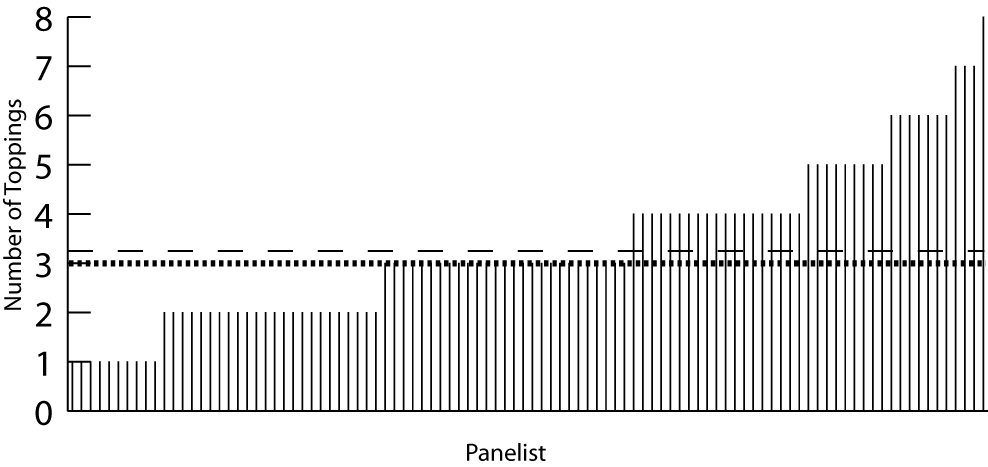
\includegraphics[width=0.9\textwidth]{./img/Figure41.png}
\end{figure}

Part 1 of the survey was completed in 20-35 minutes for each subject.  Figure~\ref{fig:pizzsize} is a histogram showing the number of compatible pairs by percentages of responses.  As mentioned above, we adjusted our threshold to 78 out of 124 panelists, which means that a proportion of people equal to 0.629 had to agree that a pair was compatible for it to be counted as an edge.  An alternative thresholding strategy could decide a threshold based on the proportion itself rather than size of the combination (essentially our method in reverse).  This would allow the investigator to say “we only want pairs accepted by 75\% of the population.”  Dangers of setting the threshold too high or too low are evident in Figure~\ref{fig:pizzsize}.  If the threshold is too strict, Type II error becomes a danger and if it is too lenient Type I error becomes a concern.  As the threshold goes up, you are more likely to miss combinations that may be acceptable.  As the threshold goes down, less compatible cliques are likely to emerge in to the results.  This risk assessment is an important aspect of the experimental design.

\begin{figure}[h!]
\caption[The distribution of responses from Part 1 of the survey.]{The distribution of responses from  Part 1 of the survey.  This shows the number of pairs that people determined were compatible.  The mean proportion was 0.50.}
\label{fig:pizzsize}
\centering
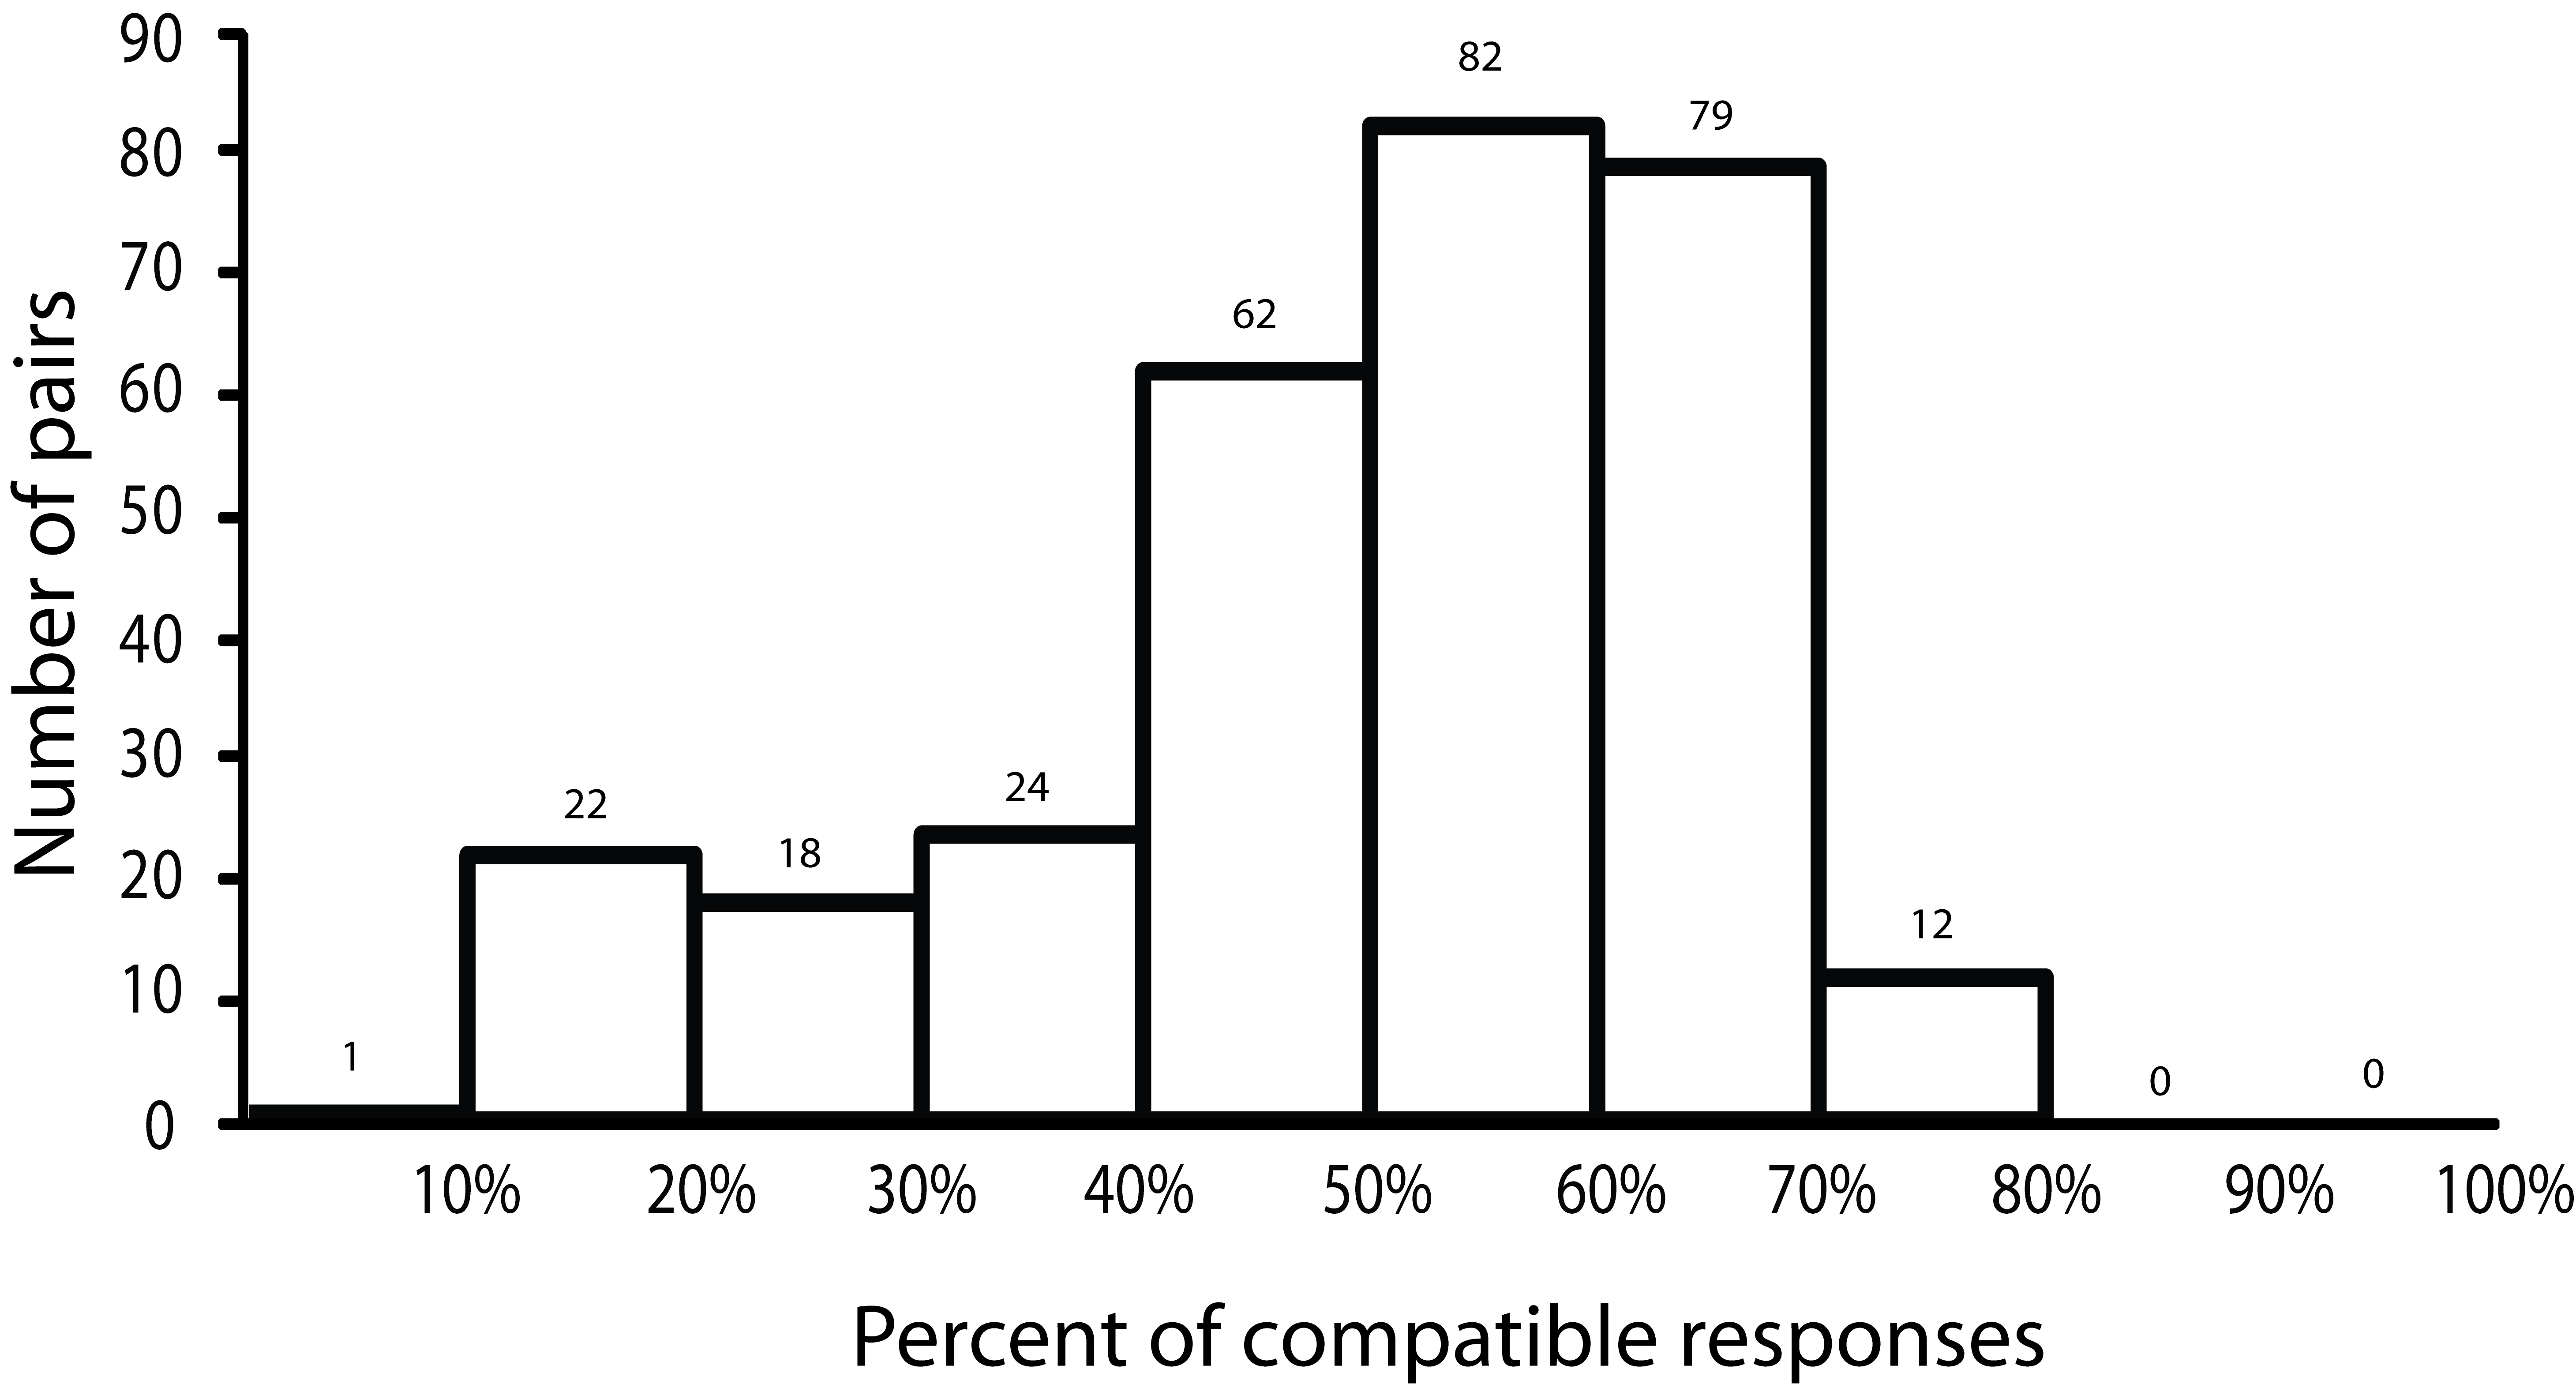
\includegraphics[width=0.9\textwidth]{./img/Figure42.png}
\end{figure}

Once our threshold was applied, 50 out of 300 compatible pairs moved forward in the analysis.  Figure~\ref{fig:pizzedge} shows a graph with edges of the 50 pairs that were used to find larger combinations of compatible pizza toppings. It is evident from this graph that weakly connected toppings like pineapple and red onion are liked in combination with few ingredients, as opposed to ingredients like pepperoni and roasted garlic.  Ingredients such as anchovy and prosciutto that are not connected to other ingredients tend to be liked, but only by themselves (or with ingredients not in our top twenty-five).  From this graph we found the complete set of non-cliques, non-maximal cliques and cliques from sizes one through six.

\begin{table}[h!b!p!]
\caption[Proportion of panelists who chose pizzas of combination sizes 1-6 and overall to be compatible.]{Proportion of panelists who chose pizzas of combination sizes 1-6 and overall to be compatible.  There is a trend to decreasing compatibility as size increases.  }
\label{tab:pizzcompat}
\centering
\begin{tabular}{cccc}
\toprule
{\bf Combination Size} & {\bf Max Cliques} & {\bf Non-max Cliques} & {\bf Non-Cliques}  \\
\midrule
1 & 0.41 & 0.68 & 0.48 \\
2 &  0.64 & 0.69 & 0.42 \\
3 &  0.66 & 0.62 & 0.36 \\
4 &  0.56 & 0.62 & 0.29 \\
5 &  0.57 & 0.58 & 0.26 \\
6 & 0.55 & 0.68 & 0.37 \\
\midrule
Overall & 0.55 & 0.65 & 0.37 \\
\bottomrule
\end{tabular}
\end{table}

The results provide evidence in favor of the SC property.  The overall proportions of YES responses for each of the three groups (non-cliques, non-maximal cliques and maximal cliques) were [0.37, 0.65, 0.55].  These proportions are broken down by combination size in Table~\ref{tab:pizzcompat}.  Maximal cliques of size one (Anchovy, Artichoke, Prosciutto, Jalapeno, Black Olive and Eggplant) were polarizing and had proportions of people who reported purchase interest to a degree more similar to that of the non-cliques than to the cliques. There is also a slight trend across all three groups which indicates that as the number of ingredients increases the probability of a combination being accepted is lower.  This is in line with trend shown in the internet pre-survey in which subjects overwhelmingly listed 1-3 ingredient pizzas as their favorites.

\begin{figure}[h!]
\caption[Edge graph based on thresholded pairwise responses from part 1]{Edge graph based on thresholded pairwise responses from part 1.  Highly connected toppings are highly compatible.}
\label{fig:pizzedge}
\centering
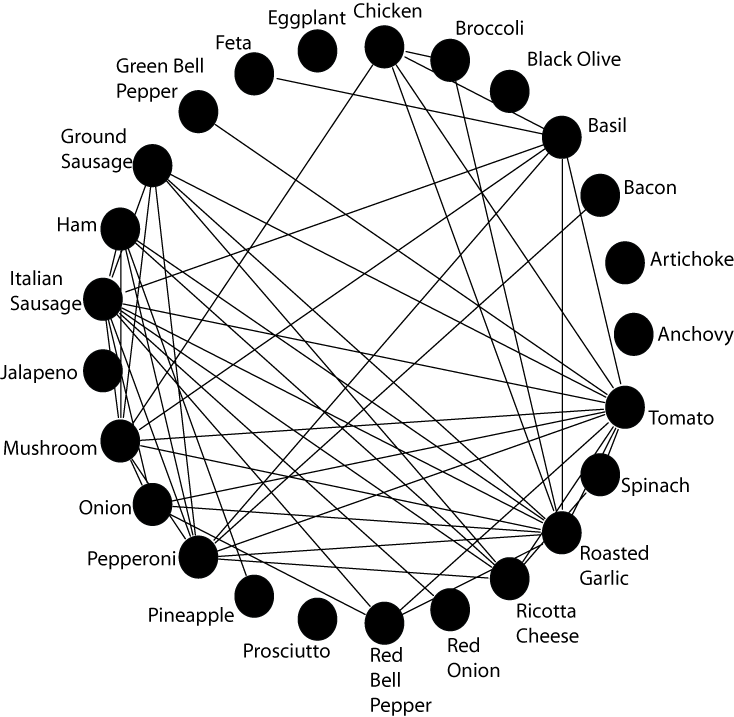
\includegraphics[width=0.9\textwidth]{./img/Figure43.png}
\end{figure}

Figure~\ref{fig:pizzdist} shows the average counts of the number of times a pizza with a given number of toppings was chosen to be compatible for each of the three groups.  As noted above, the max clique of size one is distanced from the rest of the clique responses because these ingredients are polarizing.  The Tukey quick test was designed to assess whether or not two distributions are separated.  There is no significant difference between the maximal-clique and the non-maximal clique groups.  Formal statistical tests cannot be performed to test the difference between the non-cliques and each of the clique groups because the non-parametric tests, including the Wilcox or the Tukey quick test, require that the distributions overlap.  As these distributions do not overlap, we can conclude that the distributions are in fact different and that there is evidence in support of the SC effect.  

\begin{figure}[h!]
\caption[Distribution of average counts of compatible pizzas.]{M:max cliques, C:non-max cliques, N:non-cliques.  Distribution of average counts of compatible pizzas.  Non-cliques were liked less than cliques or max cliques.  There is no difference between the non-max clique and max-clique distributions.}
\label{fig:pizzdist}
\centering
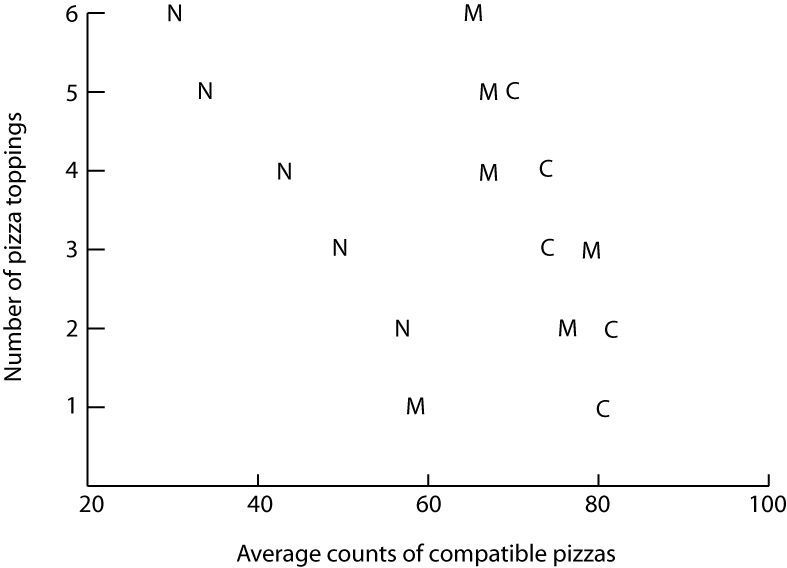
\includegraphics[width=0.9\textwidth]{./img/Figure44.png}
\end{figure}

The combinatorial approach of \citet{Ennis2010} holds promise in allowing food product developers to gain information regarding a large number of food item combinations in a cost efficient manner.  Even so, this technique rests on the crucial SC assumption that needs to be validated before this approach can be confidently employed.  Previously, SC was validated at the individual level \citep{Nestrud2010a}. The research communicated in this present paper demonstrates that SC holds in a group setting and for a different product category.  In this case, the graph theoretic tools allowed us to screen almost a quarter of a million possible combinations down to twenty-one cliques, which were then shown to be of high quality in subsequent testing.  Importantly, these results were obtained in under 30 minutes by asking respondents to generate only three hundred binary responses. 

A future project is to extend the combinatorial approach to meal design, where components from different categories (e.g. starch, protein, vegetable, dessert) are combined to create a highly compatible meal.  This would be useful in the many situations where meals are predetermined, from frozen foods and airline meals to “prix fixe” restaurant value menus and institutional settings such as military and school lunch programs.

\section{Acknowledgements}
The authors thank Effie Nestrud for laboratory assistance and Charles Fayle for invaluable and skillful programming. 

\pagebreak
\renewcommand\bibname{{REFERENCES}} %  will print "REFERENCES" instead of "BIBLIOGRAPHY"
\phantomsection
\addcontentsline{toc}{section}{References} %  adds "REFERENCES" to the table of content
\bibliographystyle{apalike}
\bibliography{library_man}  % uses the references stored in Chapter1Radar.bib